\documentclass{article}
\usepackage[utf8]{inputenc}
\usepackage[T1]{fontenc}
\usepackage[english]{babel}
\setlength{\parindent}{0pt}
\usepackage{hyperref}
\hypersetup{
    colorlinks=true,
    linkcolor=blue,
    filecolor=magenta,      
    urlcolor=cyan}
\usepackage{graphicx}
\graphicspath{ {./pic/} }

\usepackage{fourier,amssymb,microtype,amsmath,gensymb}
\newcommand{\R}{\mathbb{R}}
\usepackage{mdframed,caption,xcolor,enumitem}
\usepackage{tikz,tkz-euclide}

\title{Seminar 2 - Expenditure function}
\author{Xiaoguang Ling \\  \href{xiaoguang.ling@econ.uio.no}{xiaoguang.ling@econ.uio.no}}
\date{\today}

\begin{document}

\maketitle

%%%%%%%%%%%%%%%%%%%%%%%%%%%%%%%%%%%%%%%%%%%%%%%%%%%%%%%%%%%%%%%%%%%%%%%%%%%%%%%%%%%%%%%%%%%%%%
\section{Jehle \& Reny 1.38 - Properties of the Expenditure Function}
Verify that the expenditure function obtained from the CES direct utility function in Example 1.3 
(JR. pp.39) satisfies all the properties given in Theorem 1.7 (JR. pp.37).

\begin{mdframed}[backgroundcolor=blue!20,linecolor=white]

\textbf{Expenditure Function (JR. pp.35)}

We define the expenditure function as theminimum-value function:

$$e(p, u) \equiv \min_{x \in \R^n_+} p \cdot x$$

\textbf{THEOREM 1.7 Properties of the Expenditure Function (JR. pp.37)}

\bigskip

If $u(.)$ is continuous and strictly increasing, then $e(p, u)$ defined in (1.14) is

\begin{enumerate}
\item Zero when $u$ takes on the lowest level of utility in $\mathcal{U}$,
\item Continuous on its domain $\R^n_{++} \times \mathcal{U}$,
\item For all $p \gg 0$, strictly increasing and unbounded above in $u$,
\item Increasing in $p$,
\item Homogeneous of degree $1$ in $p$,
\item Concave in $p$.
\end{enumerate}
If, in addition, $u(.)$ is strictly quasiconcave, we have
\begin{enumerate}[start = 7]
\item Shephard’s lemma: $e(p, u)$ is differentiable in $p$ at $(p^0, u^0)$ with $p^0 \gg 0$, and
$$\frac{\partial e(p^0, u^0)}{\partial p_i} = x^h_i (p^0, u^0), \ \ \ \ i = 1, . . . , n.$$
\end{enumerate}
\end{mdframed}


%***************************************************
\subsection{}

















%%%%%%%%%%%%%%%%%%%%%%%%%%%%%%%%%%%%%%%%%%%%%%%%%%%%%%%%%%%%%%%%%%%%%%%%%%%%%%%%%%%%%%%%%%%%%%
\section{Jehle \& Reny 1.44 - Inferior and Normal goods}
In a two-good case, show that if one good is inferior, the other good must be normal.




%%%%%%%%%%%%%%%%%%%%%%%%%%%%%%%%%%%%%%%%%%%%%%%%%%%%%%%%%%%%%%%%%%%%%%%%%%%%%%%%%%%%%%%%%%%%%%
\section{Jehle \& Reny 1.51 - Substitues and Complements}
Consider the utility function, $u(x_1, x_2) = (x_1)^{1/2} + (x_2)^{1/2}$.

\begin{enumerate}[label=\alph*.]

\item Compute the demand functions, $x_i(p_1, p_2, y), \ i = 1, 2$.

\item Compute the substitution term in the Slutsky equation for the effects on $x_1$ of changes in $p_2$.

\item Classify $x_1$ and $x_2$ as (gross) complements or substitutes.

\end{enumerate}



\begin{figure}

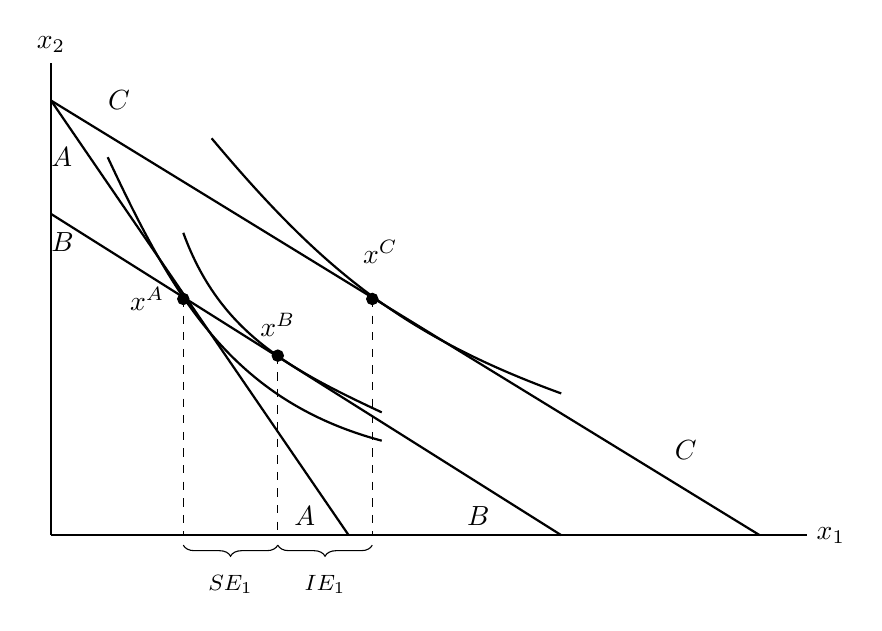
\begin{tikzpicture}[scale=1.2]

\draw [thick] (0,0) -- (8,0);
\draw [thick] (0,0) -- (0,5);
\node [right] at (8,0) {$x_1$};
\node [above] at (0,5) {$x_2$};
\draw [thick] (1.7,4.2) to [out=310,in=160] (5.4,1.5);
\draw [thick] (0.6,4) to [out=295,in=165] (3.5,1);
\draw [thick] (1.4,3.2) to [out=290,in=155] (3.5,1.3);
\node [right] at (6.5,0.9) {$C$};
\draw [thick] (0,4.6) -- (7.5,0);
\draw [thick] (0,4.6) -- (3.15,0);
\draw[dashed](1.4,2.5)--(1.4,0);
\draw[dashed](3.4,2.5)--(3.4,0);
\draw [thick] (0,3.4) -- (5.4,0);
\draw[dashed](2.4,1.9)--(2.4,0);
\node [above] at (2.4,2) {$x^B$};
\draw[fill] (2.4,1.9) circle [radius =0.06];
\node [left] at (1.3,2.5) {$x^A$};
\draw[fill] (1.4,2.5) circle [radius =0.06];
\node [right] at (3.2,3) {$x^C$};
\draw[fill] (3.4,2.5) circle [radius =0.06];
\node [right] at (0.5,4.6) {$C$};
\node [right] at (-0.1,4) {$A$};
\node [left] at (2.9,0.2) {$A$};
\node [right] at (4.3,0.2) {$B$};
\node [right] at (-0.1,3.1) {$B$};
\draw [decorate,decoration={brace,amplitude=4pt, mirror},xshift=0pt,yshift=-3pt]
(1.4,0) -- (2.4,0) node [black,midway,yshift=-.5cm] {\footnotesize $SE_1$};
\draw [decorate,decoration={brace,amplitude=4pt, mirror},xshift=0pt,yshift=-3pt]
(2.4,0) -- (3.4,0) node [black,midway,yshift=-.5cm] {\footnotesize $IE_1$};
\end{tikzpicture}
\caption{Slutsky decomposition}
\end{figure}
\end{document}